\section{Analysis}\label{sc:analysis}
In order to asses the correct progress of the rnucs-mesh workflow, a few 
analysis were performed on toy problems designed to have interaction in the 
high energy region. 

\subsection{Problem Description}
Two toy problems were identified to asses the correctness of the 
rnucs-mesh workflow. 
Toy problem I (shown in Figure \ref{TPI}) consists of a mercury rectangular prism that is 
22 cm x 44 cm x 186 cm. 

\begin{figure}[h!]
\begin{centering}
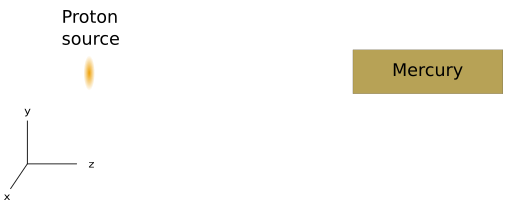
\includegraphics[width=0.60\linewidth]{../figs/mercury.png}
\caption{Planar view of Toy Problem I geometry, 22 cm  x 44 cm x 186 cm }
\label{TPI}
\end{centering}
\end{figure}
Toy problem II (shown in Figure \ref{TPII}) has a rectagular prism enclosing another rectagular
prism. 
The mercury cell has the same dimensions as those of toy problem I. The steel 
cell, which encloses the mercury, is double the size of the mercury cell. 
% Figure
% Figure
\begin{figure}[h!]
\begin{centering}
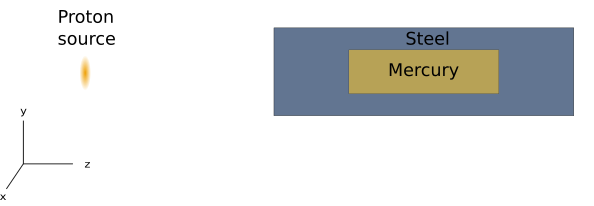
\includegraphics[width=0.70\linewidth]{../figs/mer_steel.png}
%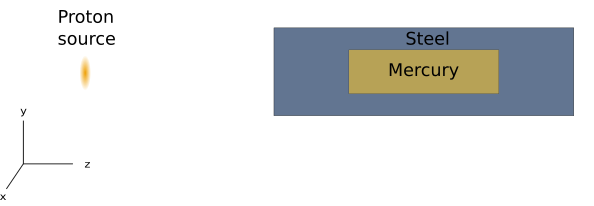
\includegraphics{../figs/mer_steel.png}
\caption{Planar view of Toy Problem II geometry, 44 cm  x 88 cm x 372 cm }
\label{TPII}
\end{centering}
\end{figure}

Both toy problems have a 1 GeV proton source located 
along the negative z direction with distributions along the x and y directions.
A total of six geometries were created, three for each toy problem. 
The first geometry was built as described above, the second geometry 
was split into 8 equal cells and the last one was split 64 equal cells.
Splitting toy problem II into 8 equal cells required some material mixing. 
Each cell in this particular geometry was assigned a steel-mercury mixture
of 3:1. 

\subsection{Workflow to Photon Emissions}
In oder to generate the spectrum file, the following steps were carried out:
\begin{itemize}
\item MCNP run 
\item Generation of 
\end{itemize}
The following runs were performed:

\begin{itemize}
  \item rnucs on cells 
  \item 1x1x1 mesh
  \item 2x2x2 mesh
  \item 4x4x4 mesh 
  \item 2x2x2 split
  \item 4x4x4 split
\end{itemize}

Each mesh covered the entire geometry and was uniformly distributed. 
Splitting toy problem II into 8 equal parts required the mixed material to be created. 
The mixed material was 3:1 ratio of steel and mercury. 
p
Each case mentioned below was run with 1E6 history particles. 
\subsection{Activation}

An activation calculation was done for each run for a set of irradiation history. 




\newpage
